\documentclass[times, doublespace]{anzsauth}
\usepackage{moreverb}
\usepackage{url}
\usepackage{grffile}
\usepackage{lineno}
% \usepackage{lmodern}
\usepackage{lipsum}
\usepackage[UKenglish]{isodate}
\usepackage{float}
\usepackage{subcaption}
\usepackage{algorithm}
\usepackage{algpseudocode}
% \newfloat{lstfloat}{htbp}{lop}
% \floatname{lstfloat}{Listing}
% \def\lstfloatautorefname{Listing}

% \doublespace
\usepackage{afterpage}



\newcommand{\bv}{\boldsymbol{v}}
\newcommand{\bz}{\boldsymbol{z}}
\newcommand{\bw}{\boldsymbol{w}}
\newcommand{\bR}{\boldsymbol{R}}
\newcommand{\bT}{\boldsymbol{T}}
\newcommand{\br}{\boldsymbol{r}}
\newcommand{\btheta}{\boldsymbol{\theta}}

\newcommand{\rt}{real-time\ }

\def\volumeyear{2020}
\linenumbers

\begin{document}
\cleanlookdateon
\runningheads{Modelling the travel time of transit vehicles}{TOM~ELLIOTT AND THOMAS~LUMLEY}
\title{
    Modelling the travel time of transit vehicles in \rt through a GTFS-based road network
    using GPS vehicle locations
}

% Modelling transit vehicles to estimate the \rt traffic conditions in a public transport network}
\author{Tom Elliott\corrauth~and~Thomas~Lumley}
\affiliation{University of Auckland}
\address{
    Department of Statistics, University of Auckland,
    Auckland 1142, New Zealand\\
    Email: \texttt{tom.elliott@auckland.ac.nz}
}
\ack{
    We would like to thank Auckland Transport for providing free,
    open access to the \rt data; and the Centre for e-Research at the
    University of Auckland for providing and maintaining the virtual
    machine used in our work.
}

\begin{abstract}
Predicting the arrival time of a transit vehicle involves not only
knowledge of its current position and schedule adherence,
but also traffic conditions along the remainder of the route.
Road networks are dynamic
and can quickly change from free-flowing to highly congested,
which impacts the arrival time of transit vehicles,
particularly buses which often share the road with other vehicles,
so reliable predictions need to account for \rt and future traffic conditions.
The first step in this process is to construct a framework with which road state
(traffic conditions) can be estimated using \rt transit vehicle position data.
Our proposed framework implements a vehicle model using a particle filter
to estimate road travel times,
which are used in a second model to estimate \rt traffic conditions.
Although development and testing took place in Auckland, New Zealand,
we generalised each component to make the framework compatible
with other public transport systems around the world.
We demonstrate the \rt feasibility and performance of our approach in real-time,
where a combination of \textsf{R} and \textsf{C++} was used to obtain the necessary performance results.
Future work will use these estimated traffic conditions
in combination with historical data to obtain reliable
arrival time predictions of transit vehicles.
\end{abstract}

\keywords{particle filter; transit modelling;
          transit networks; applications; gtfs}

\maketitle

\section{Introduction}
\label{sec:intro}


In public transport, \rt information (RTI)---%
most notably estimated times of arrival (ETAs)---%
keeps transport users informed of changes to their commute,
allowing them to plan their journey accordingly.
Previous research has shown that perceived waiting time is less
when arrival time information is available \citep{TCRP_2003b};
however, in Auckland, RTI is highly unreliable,
leading to frustration and ultimately deterring public transport users.
Inaccurate ETAs are the primary source of this frustration,
as they fluctuate---sometimes dramatically---over time.
While unpredictable changes to traffic conditions may cause this,
it can equally be due to poor schedule calibration.
Furthermore, buses are shown as \emph{on-time}
if they are not present in the \rt system and
the service provider has not manually cancelled them,
in which case ETAs are based solely on scheduled arrival times.
Once the scheduled arrival time has passed,
the service is removed from the \rt board,
leaving passengers unsure as to when---if at all---their bus will show up,
a phenomenon referred to as `ghost buses' by transport bloggers.


Arrival time prediction is only as reliable as the underlying model,
and while considerable work has gone into developing public transport vehicle models
\citep{Cathey_2003,Jeong_2005,Yu_2011,Hans_2015},
many public transport providers---notably Auckland Transport---use no formal model.
Instead, ETAs are based solely on the scheduled arrival time
adjusted by the vehicle's arrival or departure delay at the most recent stop,
\emph{if available}.
This method assumes that the schedule is accurate
and there is no unusual congestion along the route.
Neither of these is a valid assumption,
particularly in our test area of Auckland, New Zealand,
where infrastructure for buses (such as priority lanes) is limited,
and bus drivers do not actively adhere to the schedule.
A more robust modelling and prediction framework
based on \rt congestion information would avoid making these assumptions.
Such a framework should consist of a robust vehicle model to estimate the position and speed
of transit vehicles from \rt GPS data,
and a means of combining speed information from vehicles
to model traffic flow.
This information can then be used to improve arrival time predictions.


Several vehicle modelling approaches were explored,
including the Kalman filter \citep{Dailey_2001,Cathey_2003},
machine learning models \citep{Yu_2006,Chang_2010},
and the particle filter \citep{Hans_2015},
which has proven itself as a robust option for
\rt vehicle tracking applications
\citep{Gustafsson_2002,Davidson_2011}.
\cite{Ulmke_2006} compared both a Gaussian sum approximation and a particle filter
to track a vehicle in real-time,
and although not their primary aim,
showed how the particle filter behaved better in some difficult situations.
In particular, the particle filter accurately estimated the \emph{uncertainty}
of the vehicle's location when the observations were unavailable for a time.
This situation often occurs with transit data---%
the bus may be stopped at a bus stop, or it could be continuing along the route but,
for some other reason, failing to report its position.
Choosing to implement a particle filter has allowed us
to develop a simple, flexible framework
which is robust to the type of data we expect to observe.


The second component of our framework
involves estimating traffic conditions throughout the transport network
using the information obtained from the vehicle model.
\cite{Yu_2010} improved prediction accuracy by using the travel times
of previous buses travelling along the same route.
A similar method presented by \cite{Hans_2015}
used headway, the time between consecutive vehicles at a point on the route,
as a predictor of travel time.
Since these approaches only work well on high-frequency routes,
\cite{Yu_2011} showed further improvements by combining travel times
from several routes;
however, their method was limited to predefined converging routes.
In general, however, no comprehensive network modelling approach has been proposed using
only GPS position data to model and account for congestion when estimating arrival times.

In this paper, we propose a simple framework for modelling transit vehicles and predicting
their arrival times in real-time.
Section~\ref{sec:gtfs} describes how we constructed a transit network,
allowing us to model travel times along physical roads,
while Section~\ref{sec:models} presents two \rt models---%
one for each of the vehicle and network states---%
with the primary goal of estimating \rt traffic states throughout the network.
Finally, we discuss the \rt feasibility and performance
of the particle filter in Section~\ref{sec:rt}.


\section{Working with \rt transit data}
\label{sec:gtfs}


GTFS (general transit feed specification)
is an API (application programming interface) specification for transit data
detailing how it should be organised,
making access easier for application developers.
GTFS, developed and maintained by Google \citep{GoogleDevelopers_2006},
% who use it in Google Maps Transit Directions,
is used by over 1100~transit providers around the world
(sourced from \url{http://transitfeeds.com} on August 2019),
including here in Auckland, New Zealand.
An advantage of this standardised format is that,
provided an application depends solely on GTFS data,
after developing it locally in Auckland it will be deployable to any other GTFS-based
public transport system with minimal modification.


There are two components to GTFS.
The first, \emph{GTFS static}, includes information about:
\begin{itemize}
\item \emph{stops}, a physical location where passengers can embark and disembark the vehicle;
\item \emph{routes}, a sequence of two or more stops displayed as a single service;
\item \emph{trips}, an instance of a route occurring at a specific time of day;
\item \emph{schedules}, specifying the arrival (and departure) times for each bus at each of its stops;
\item and \emph{shapes}, the sequence of points defining a vehicle's path along a route.
\end{itemize}
The second component, \emph{GTFS-realtime},
is only available in a subset of providers due to the requirement of
on-board GPS tracking devices and a central server.
It provides a standardised format for sharing vehicle positions and trip delays,
which developers access via an API for use in \rt applications.

As mentioned in Section~\ref{sec:intro},
there are some fundamental issues with the arrival time prediction method currently
deployed in Auckland,
which is based entirely on \emph{GTFS-realtime} trip updates---%
vehicle positions are used only to display \emph{where} the bus is.
Vehicles report a trip update,
which includes the delay between scheduled and actual arrival time,
when they arrive at or depart from a stop.
The delay is then propagated to all future stops to update their ETAs,
as demonstrated in Figure~\ref{fig:gtfs-delays}.
As already mentioned, this assumes that the schedule is well-calibrated
and that the time between stops
is representative of the real-world travel time between them.
Figure~\ref{fig:gtfs-delays} demonstrates the fallibility of this prediction method,
where we see the incremental lateness causing the passenger's ETA to
jump each time the bus arrives at a stop.
By using \rt travel time information,
we can better predict the travel time between stops,
from which more accurate and, ideally, more reliable arrival esimates
can be made.


\begin{figure}[tb]
    \centering
    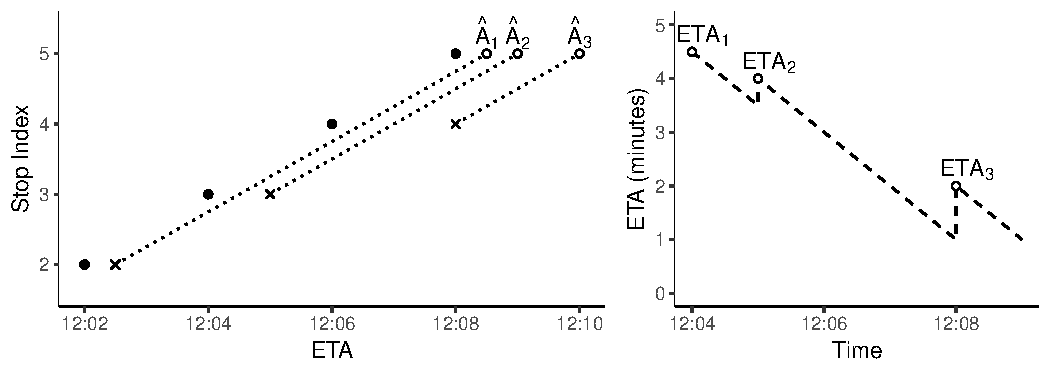
\includegraphics[width=0.8\textwidth]{figures/02_gtfs_delays.pdf}
    \caption{
        On the left, scheduled arrival times are shown as solid points,
        for several stops along a route. The actual arrival times
        are shown with crosses,
        and the GTFS-based ETAs for stop 5, $\{\hat A_1, \hat A_2, \hat A_3\}$, are shown.
        On the right,
        for a passenger arriving at stop 5 at 12:04,
        ETA predictions
        $\mathrm{ETA}_j = \mathrm{Time} - \hat A_j$ are shown
        to demonstrate the fluctuation in
        arrival time as the bus arrives at each stop.
    }
    \label{fig:gtfs-delays}
\end{figure}



\subsection{Transit network construction}
\label{sec:network_build}

The primary predictor of arrival time is
the travel time along roads between where the bus is \emph{now},
and the stop where a passenger waits.
In most applications, however, this vital information is unavailable, at least directly.
In order to compute travel times efficiently
and make use of all available data pooled across multiple routes,
we constructed a \emph{road network},
allowing us to model roads directly,
such that every bus travelling along a road contributes to its state,
which can, in turn, be used to predict travel times for all upcoming buses
travelling along the same road,
irrespective of the route they are servicing.


Constructing the transit network involved splitting routes
into spatially identifiable segments,
each representative of a physical road,
using bus stops as nodes in the network
and the connecting roads as edges
(Figure~\ref{fig:network_creation}).
In this way, routes that service the same subsequence of stops
all contribute to traffic flow information for the connecting roads.
Although there are several drawbacks to this method,
such as road segment overlaps where routes merge between stops,
our approach is sufficient for assessing the \rt
feasibility of our proposed prediction framework.



\begin{figure}[tb]
    \centering
    \begin{subfigure}{0.7\textwidth}
        \centering
        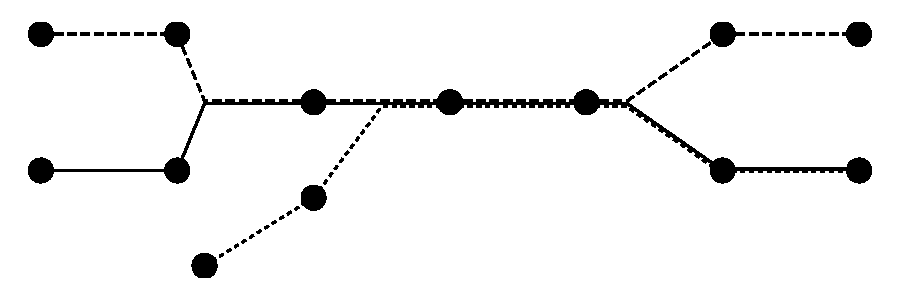
\includegraphics[width=0.9\textwidth]{figures/02_network_segments_1.pdf}
        \caption{Raw GTFS route shapes}
        \label{fig:network_creation_1}
    \end{subfigure} \\
    \begin{subfigure}{0.7\textwidth}
        \centering
        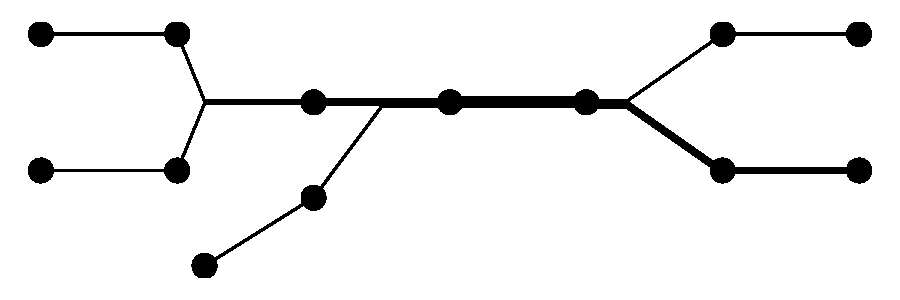
\includegraphics[width=0.9\textwidth]{figures/02_network_segments_2.pdf}
        \caption{GTFS-based road network}
        \label{fig:network_creation_2}
    \end{subfigure}
    \caption{
        Bus stops (shown as dots above) can be serviced by more than one route,
        as shown in (a), with different line types representing three separate routes.
        The constructed road network, using stops as nodes, is shown in (b),
        in which the connecting lines represent physical road segments,
        with line width proportional to the number of individual routes
        travelling along that road.
    }
    \label{fig:network_creation}
\end{figure}


\subsection{Real-time vehicle locations}
\label{sec:realtime_data}

\emph{GTFS-realtime} provides the positions of vehicles in a transit network.
The data consists of the time $t_k$ that the position was last updated,
the GPS position of the vehicle, $\bY_k$,
and information about the serviced trip.
In Auckland, vehicle positions are updated with a frequency
of anywhere between 10~seconds and several minutes,
so there is often considerable uncertainty about a vehicle's intermediate trajectory,
in particular when there are one or more bus stops along the way.
It is also possible for a bus to remain stationary,
such as when there is heavy congestion,
so the number of possible trajectories rapidly increases with
the time between observations.


An important consideration regarding Auckland Transport's \rt implementation is that
buses are programmed to report their location when arriving at or departing from
bus stops, as well as some major intersections.
To further complicate this,
these positions can be pre-emptive,
for example when approaching a queue of traffic at an intersection:
the way-point may trigger before the bus physically gets to it,
so consecutive observations may show what appears to be a bus travelling backwards.
To handle this, we compute the approximate distance travelled, $\tilde x_k$,
of the vehicle by finding the nearest point on the path to the observation;
if this has decreased, we reject the current state (based on the pre-emptive observation)
and reset the vehicle
to its previous state before continuing.
So at the cost of losing one (likely invalid) observation,
we can improve predictive performance
when this event occurs.


\section{The models}
\label{sec:models}

Real-time tracking applications often use
a Bayesian filtering approach,
or recursive Bayesian estimation,
in which the data is processed sequentially instead of all at once,
reducing computational demands
\citep{Anderson_2012}.
These models assume an underlying Markov process with state $\boldsymbol{\mathcal{X}}_k$,
an $n\times1$ column vector,
with system noise $\boldsymbol{\omega}_k\sim\mathrm{N}(\boldsymbol{0},\mathcal{Q})$
of which observations $\boldsymbol{\mathcal{Y}}_k$,
an $m\times1$ column vector, are made
with error $\boldsymbol{\nu}_k\sim\mathrm{N}(\boldsymbol{0},\mathcal{R})$,
giving the following general model:
\begin{equation}
\label{eq:rbe_model}
\begin{split}
\boldsymbol{\mathcal{X}}_k &= f(\boldsymbol{\mathcal{X}}_{k-1}, \boldsymbol{\omega}_k), \\
\boldsymbol{\mathcal{Y}}_k &= h(\boldsymbol{\mathcal{X}}_k) + \boldsymbol{\nu}_k.
\end{split}
\end{equation}
The transition function $f:\mathbb{R}^n\mapsto\mathbb{R}^n$
describes the relationship between consecutive states,
while the measurement function $h:\mathbb{R}^n\mapsto\mathbb{R}^m$ is a deterministic function
mapping the underlying state to the observable state,
of which noisy measurements are made.



The following sections describe two Bayesian filters used in this application.
The first, implemented using a particle filter, estimates vehicle states
with the primary goal of estimating road travel times from a sequence of GPS positions.
The second uses these travel times to update road states
and is implemented using an \emph{information filter},
a variant of the Kalman filter \citep{Anderson_2012}.



\subsection{Real-time vehicle model}
\label{sec:pf}

The underlying vehicle state at time $t_k$ consists of
the vehicle's distance travelled $x_k$ in meters along the route and
its speed $\dot x_k$ in meters per second.
These are combined into the state vector
$\bX_k = \left[x_k\ \dot x_k\right]^\top$,
of which observations $\bY_k$ are made using a GPS
with error $\omega^2$,
giving the longitude $\lambda_k$ and latitude $\phi_k$ of the vehicle
as $\bY_k = \left[\lambda_k\ \phi_k \right]^\top$.
We use a particle filter to estimate $\bX_k$
due to its flexibility and proven robustness
in recent vehicle modelling applications \citep{Ulmke_2006,Hans_2015}.
It also allows us to estimate travel times
$\bz = (z_1,\ldots,z_L)^\top$, in seconds, along road segments
as the vehicle traverses the route.


The primary advantage of the particle filter is its handling of multimodality,
as demonstrated in Figure~\ref{fig:pf_state_predict},
which is a common feature of the proposal distribution, particularly around bus stops.
Another advantage is that the likelihood function is intuitive, based
on the physical distance between the vehicle observation and the state's
estimate of the actual location, $h(\bX_k)$ (Section~\ref{sec:pf_update}).
Conversely, particle filter methods are computationally demanding,
requiring an increasing number of particles as model complexity and
the number of parameters increases \citep{Carpenter_1999}.
Section~\ref{sec:rt} describes our implementation of the particle filter
and its \rt performance.

\begin{figure}[p]
    \centering
    \begin{subfigure}[t]{1\textwidth}
        \centering
        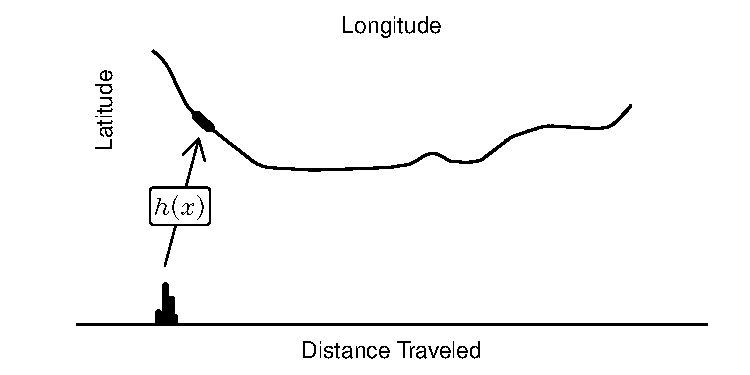
\includegraphics[width=0.7\textwidth]{figures/03_particle_filter_1.pdf}
        \caption{
            Vehicle state is mapped to observation space by the
            measurement function $h$.
        }
        \label{fig:pf_state_prev}
    \end{subfigure}\\
    \begin{subfigure}[t]{0.9\textwidth}
        \centering
        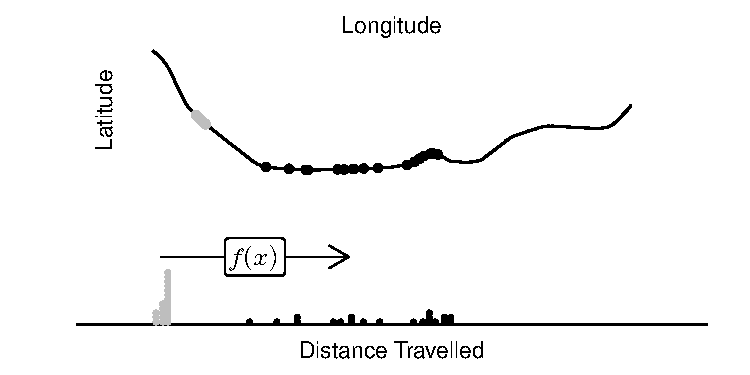
\includegraphics[width=0.7\textwidth]{figures/03_particle_filter_2.pdf}
        \caption{
            The transition function $f$ predicts the future state
            of each particle.
        }
        \label{fig:pf_state_predict}
    \end{subfigure}\\
    \begin{subfigure}[t]{0.9\textwidth}
        \centering
        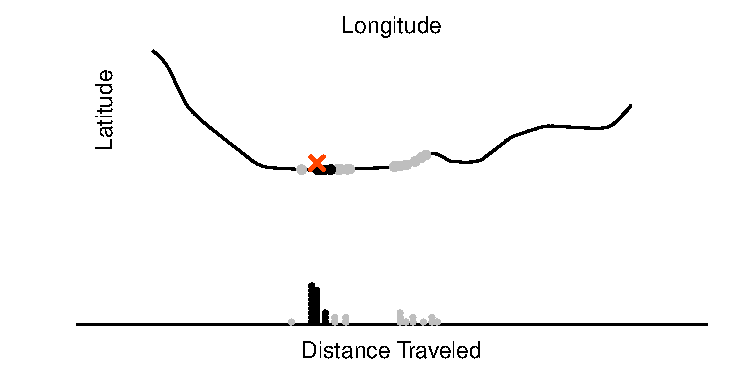
\includegraphics[width=0.7\textwidth]{figures/03_particle_filter_4.pdf}
        \caption{
            The state is updated by resampling with likelihood weights based on the distance
            between the particle and the observation, shown as a (red) cross.
        }
        \label{fig:pf_state_predict2}
    \end{subfigure}
    \caption{
        The particle filter approximates vehicle state using a set of
        discrete points (a), which are each mutated independently (b)
        to predict the next state.
        The measurement function $h$ maps each particle state
        to a GPS coordinate (a),
        which can be compared to the observed location (c)
        to calculate each particle's likelihood to compute resampling weights.
    }
    \label{fig:pf_state}
\end{figure}

\afterpage{\clearpage}

In a particle filter, the posterior distribution of the state at time $t_{k-1}$
is represented by a set of discrete points, or particles, (Figure~\ref{fig:pf_state_prev}),
each with an associated weight $W_{k-1}^{(i)}$.
The state is expressed using the Dirac delta function $\dot\delta(\cdot)$,
\begin{equation*}
p(\bX_{k-1} | \bY_{1:k-1}) \approx
    \sum_{i=1}^N W_{k-1}^{(i)} \dot\delta(\bX_{k-1} - \bX_{k-1}^{(i)}),
\end{equation*}
which is updated of \emph{mutated} by applying the transition function $f$
to each particle independently (Figure~\ref{fig:pf_state_predict}),
giving us the proposal distribution
\begin{equation*}
p(\bX_k | \bX_{k-1}) \approx
    \sum_{i=1}^N W_{k-1}^{(i)} \dot\delta(\bX_{k} - f(\bX_{k-1}^{(i)}, \boldsymbol{\psi})),
\end{equation*}
where $\boldsymbol{\psi}$ is a vector containing all of the necessary model parameters
(Section~\ref{sec:pf_prediction}).
After mutation,
the state is updated by reweighting the particles using the likelihood $p(\bY_k | \bX_k^{(i)})$
(Section~\ref{sec:pf_update}) and standardising so $\sum_{i=1}^N W_k^{(i)} = 1$,
\begin{equation*}
W_k^{(i)} = \frac{W_{k-1}^{(i)} p(\bY_k | \bX_k^{(i)})}{
    \sum_{j=1}^N W_{k-1}^{(j)} p(\bY_k | \bX_k^{(j)})
},
\end{equation*}
which leads to the final posterior state estimate
\begin{equation*}
p(\bX_k | \bY_k) \approx
    \sum_{i=1}^N W_{k}^{(i)} \dot\delta(\bX_{k} - \bX_{k}^{(i)}).
\end{equation*}

One problem with particle filters is degeneration:
when the particles become too spread out with respect to the predictive distribution,
the weight will be concentrated on to just a few of them.
This occurs naturally over time, but the rate at which it does so depends
on the relationship between how well the transition function predicts future states
and the variance of those predictions (system noise).
If left unchecked, the predictive distribution reaches a point
where all particles have weights which are effectively zero,
at which point we say the particle filter has degenerated.
To avoid this situation,
particle filters use \emph{importance resampling}
using importance weights $\{W_k^{(1)}, \ldots, W_k^{(N)}\}$,
thereby removing improbable particles and replacing them with more probable ones,
as demonstrated in Figure~\ref{fig:pf_state_predict2}.
However, resampling requires sorting $N$ particles,
which is of $\mathcal{O}(N\log N)$ complexity,
so to reduce computational costs, resampling is performed only when
the effective sample size $N_{\text{eff}} = 1 / \sum_i (W_k^{(i)})^2$
falls below a specified threshold $N_{\text{thres}}$
\citep{Gustafsson_2002}.
We used a fixed threshold value of $N_{\text{thres}} = N/4$
for the current work.


\subsubsection{Vehicle transition function}
\label{sec:pf_prediction}

The particle filter provides us with a flexible method
with which to model bus behaviour.
Currently, this model includes:
\begin{enumerate}
\item non-constant speed along roads (between observations), and
\item bus stop behaviour, (optional stopping and wait times while passengers board and disembark).
\end{enumerate}
The transition function consists of two models,
one for each of the above behaviours.
The first models the speed and distance travelled by the vehicle,
\begin{equation}
\label{eq:trans_newton}
\bX_k^{(i)} = f(\bX_{k-1}^{(i)}, \delta_k, \epsilon_k^{(i)}) =
    \begin{bmatrix}
        x_{k-1}^{(i)} + \delta_k(\dot x_{k-1}^{(i)} + \epsilon_k^{(i)}) \\
        \dot x_{k-1}^{(i)} + \epsilon_k^{(i)}
    \end{bmatrix},
\end{equation}
where $\delta_k = t_k - t_{k-1}$
and $\epsilon_k^{(i)}\sim\mathrm{N}_T(0, \sigma^2)$, truncated to the interval
$(-\dot x_{k-1}^{(i)}, 30 - \dot x_{k-1}^{(i)})$
to ensure vehicle speed is always positive and less than 30~m/s
(approximately 110~km/h).


The second vehicle behaviour requires a model of bus stop wait times.
When approaching stop $j$,
the vehicle stops with probability $\pi_j$.
If it does not stop, the remaining travel time $\delta_k$ is unaltered;
otherwise, the bus waits for a minimum of $\gamma$ seconds---%
accounting for deceleration, opening and closing of doors, and acceleration
\citep{Hans_2015}---and then waits while passengers board and disembark,
which we assume to follow an exponential distribution with mean $\tau_j$.
Stopping behaviour is expressed in the following model:
\begin{equation}
\label{eq:trans_stop}
\begin{split}
p_j^{(i)} &\sim \mathrm{Bernoulli}(\pi_j), \\
\tilde d_j^{(i)} &\sim \mathrm{Exponential}(\tau_j), \\
d_j^{(i)} &= p_j^{(i)}(\gamma + \tilde d_j^{(i)}),
\end{split}
\end{equation}
using constant values of $\pi_j = 0.5$ and $\tau_j = 10$~seconds for all stops;
if available, historical dwell time information can easily be used
to specify each $\tau_j$,
or even replace the exponential prior altogether.
As it stands, we found these values to be vague enough that
the actual vehicle trajectory was sampled by enough of the particles
to prevent degeneration of the filter;
the consequence being increased variance of travel time estimates.


The model components are implemented as an algorithm,
in which (\ref{eq:trans_newton}) is evaluated iteratively one second at a time,
each step decreasing $\delta_k^{(i)}$ by one second,
after initialising $\delta_k^{(i)} = \delta_k$.
% To allow non-constant speed between observations,
We also re-sampled
$\epsilon_k^{(i)}$ each second
to allow the particle's speed to vary between observations.
This iterative approach allows the particle to approach the next stop,
at which point (\ref{eq:trans_stop}) is evaluated for the particle
and the dwell time subtracted from $\delta_k^{(i)}$.
This process continues until $\delta_k^{(i)}$ reaches zero.
The algorithm also keeps track of each particle's travel time $z_\ell^{(i)}$
along each segment $\ell$ of the route,
storing the times so that the posterior distribution of travel time
can be computed once all particles have completed segment $\ell$:
\begin{equation}
\label{eq:post_tt}
p(z_\ell | \bY_{1:k}) \approx
    \sum_{i=1}^N W_k^{(i)} \dot\delta(z_\ell - z_\ell^{(i)}).
\end{equation}



\subsubsection{Updating state using the observation likelihood}
\label{sec:pf_update}

Computing the likelihood of the observation given a particle state,
$p(\bY_k|\bX_k^{(i)})$,
uses the measurement function $h$ and
a \emph{geographical projection} function $g$ to allow comparison of $\bY_k$,
a GPS observation, with $\bX_k$,
which includes the distance, in meters, travelled along the route.

The measurement function $h$ computes GPS coordinates by using the
shape information provided by GTFS and travelling $x_k$ meters along
this two-dimensional line.
Meanwhile, we use the \emph{Equirectangular projection} \citep{Snyder_1998},
$\br = g(\bY_1 | \bY_0)$,
such that the magnitude of $\boldsymbol{r}$ is equal to the physical distance
between $\bY_0$ and $\bY_1$ and both dimensions are in meters.
Let $\bY_i = [\lambda_i, \psi_i]^\top$,
with $\lambda_i$ and $\psi_i$ measured in radians,
and $R$ is the Earth's radius, in meters, then
\begin{equation*}
\br =
g(\bY_1 | \bY_0) =
    \begin{bmatrix}
        r_1 \\ r_2
    \end{bmatrix} =
    R \begin{bmatrix}
        (\lambda_1 - \lambda_0)\cos\phi_0 \\
        \phi_1 - \phi_0
    \end{bmatrix},
\end{equation*}
and, more importantly, the geographical distance $\mathcal{D}$ between the two
GPS coordinates is given by
\begin{equation}
\label{eq:dist}
\mathcal{D}(\bY_0, \bY_1) = ||g(\bY_0 | \bY_1)|| = \sqrt{r_1^2 + r_2^2}.
\end{equation}


Now we assume GPS observations have a known error of $\omega^2$ meters,
and that \mbox{$\br \sim \mathrm{N}(\boldsymbol{0}, \omega^2\mathbf{I})$},
allowing us to express $\br$ in terms of two independent
standard normal random variables $z_1, z_2 \sim \mathrm{N}(0,1)$.
Now the distance between a vehicle observation $\bY_k$
and a state $\bX_k$, using (\ref{eq:dist}) and the measurement function $h$,
is expressed as
\begin{equation}
\label{eq:obs_dist}
\mathcal{D}(\bY_k, h(\bX_k)) = \sqrt{r_{k1}^2 + r_{k2}^2}
    = \sqrt{(\omega z_1)^2 + (\omega z_2)^2}
    = \sqrt{\omega^2 (z_1^2 + z_2^2)}.
\end{equation}

Finally, the sum of two independent
standard normal random variables has a Chi-square distribution with two degrees of freedom,
which is also an exponential distribution with rate~$\frac{1}{2}$,
and if $Z \sim \mathrm{Exponential}(\theta)$ then
$cZ \sim \mathrm{Exponential}(\frac{\theta}{c})$;
therefore, the \emph{squared} distance from (\ref{eq:obs_dist}) is distributed as
\begin{equation}
\label{eq:obs_exp}
\mathcal{D}(\bY_k, h(\bX_k))^2 =
\omega^2(z_1^2 + z_2^2) \sim \mathrm{Exponential}\left(\frac{1}{2\omega^2}\right).
\end{equation}

The likelihood of the observation $\bY_k$ given a state estimate $\bX_k^{(i)}$
can now be expressed using (\ref{eq:obs_exp})
and the probability density function of the exponential distribution,
\begin{equation}
\label{eq:lhood}
p(\bY_k | \bX_k^{(i)}, \omega) =
\frac{1}{2\omega^2}\exp\left\{
    -\frac{\mathcal{D}(\bY_k, h(\bX_k^{(i)}))^2}{2\omega^2}
\right\},
\end{equation}
where the distance between two GPS coordinates is easily computed,
allowing for fast evaluation of (\ref{eq:lhood}) within the particle filter algorithm.


It is worth noting that this representation of the likelihood is only
possible due to the discrete nature of the particle filter state estimate;
the Kalman filter---which has often been used for transit vehicle tracking---%
uses the measurement \emph{matrix}, requiring a linear
transformation between the state and its observations.
To do so, applications first estimate the \emph{observed distance travelled}
by snapping the GPS observations to the route,
which introduces unnecessary error and uncertainty into the model.
Our approach avoids this, which makes it more stable in locations where two
parts of the route are close to each other,
such as at loops, where a single GPS observation might have two likely ``snapping'' points.


\subsection{Network model}
\label{sec:kf}

The primary objective of the network model is to estimate the \rt traffic conditions
(travel time) along roads in the transit network
and make short-term forecasts for estimating arrival times.
In this paper, we model each road segment independently,
as excluding correlations not only simplifies the model to a one-dimensional Kalman filter,
but it also means computations can be run in parallel,
further improving the real-time performance of the model.


The network state $\boldsymbol\theta_c = \{\theta_c^\ell\}_{\ell = 1}^L$ is the travel time
of transit vehicles along road segment $\ell$ at time $t_c$,
of which observations $Z_{c\ell}^{m}$
are obtained from the particle filter for vehicle $m$ at time $t_c$,
as defined in (\ref{eq:post_tt}), such that
(after adding the $m$ superscript to identify unique vehicles),
\begin{equation}
\label{eq:tt_obs_mean}
Z_{c\ell}^{m} = \mathrm{E}(z_{\ell}^{m} | \bY^m_{1:c}) =
\sum_{i=1}^N (W_c^{(i)})^m (z_\ell^{(i)})^{m}.
\end{equation}
The measurement error is also estimated from the particle filter,
\begin{equation}
\label{eq:tt_obs_err}
R_{c\ell}^m = \mathrm{var}(z_{\ell}^{m} | \bY^m_{1:c}) =
\sum_{i=1}^N (W_c^{(i)})^m \left((z_\ell^{(i)})^{m} - Z_{c\ell}^{m}\right)^2.
\end{equation}

The model of travel times becomes a simple reduction of (\ref{eq:rbe_model})
to the one-dimensional case,
with $f$ and $h$ both unity,
system noise $v_{c\ell} \sim \mathrm{N}(0, \nu_\ell^2)$,
where $\nu_\ell^2$ is the average change in travel time per second
along road segment $\ell$,
the observation error $e_{c\ell}^{m} \sim \mathrm{N}(0, R_{c\ell}^{m})$,
and $\Delta_c = t_c - t_{c-1}$:
\begin{equation*}
\begin{split}
\theta_c^\ell &= \theta_{c-1}^\ell + \Delta_{c\ell} v_{c\ell} \\
Z_{c\ell}^{m} &= \theta_c^\ell + e_{c\ell}^{m}.
\end{split}
\end{equation*}


Since multiple vehicles can travel along a road simultaneously,
we used an information filter to implement the network model.
The information filter is a transformation of the Kalman filter in which the
\emph{information matrix} and \emph{information vector} are used in place of
the covariance matrix and state vector, respectively,
allowing multiple observations to be added together to update the state
in a single iteration.


The state at time $t_{c-1}$ is parameterised by its mean and variance,
conditional on $\boldsymbol{Z}_{1:c-1,\ell}$,
the data from all vehicles up until time $t_{c-1}$,
\begin{equation*}
\hat \theta_{c-1|c-1}^\ell =
\mathrm{E}(\theta_{c-1}^\ell | \boldsymbol{Z}_{1:c-1,\ell})
\quad\text{and}\quad
P_{c-1|c-1}^\ell =
\mathrm{var}(\theta_{c-1}^\ell | \boldsymbol{Z}_{1:c-1,\ell}),
\end{equation*}
respectively,
which are predicted from the previous state estimate using the predictive model
\begin{align*}
\label{eq:kf_transition}
\hat \theta^\ell_{c|c-1} &= \hat \theta^\ell_{c-1|c-1}, \\
P^\ell_{c|c-1} &= P^\ell_{c-1|c-1} + (\Delta_{c\ell} \nu_{c\ell})^2.
\end{align*}

For the update step, the parameters are transformed into an information
space parameterised by the information matrix $U^\ell_c = (P_{c|c-1}^\ell)^{-1}$
and the information vector $u^\ell_c~=~\hat \theta^\ell_{c|c-1} (P^\ell_{c|c-1})^{-1}$.
The travel time estimate of vehicle $m$ along segment $\ell$,
along with its uncertainty,
as defined in (\ref{eq:tt_obs_mean}) and (\ref{eq:tt_obs_err}), respectively,
are transformed to a measurement information covariance matrix
$B_{c\ell}^{m}~=~(R_{c\ell}^m)^{-2}$
and measurement information vector $b_{c\ell}^{m}~=~Z_{c\ell}^{m} (R_{c\ell}^{m})^{-2}$.
The total information is the sum of the information over all $M_{c\ell}$ vehicles
that traversed segment $\ell$ in the time interval $(t_{c-1}, t_c]$,
so the update equations are simply
\begin{align*}
U^\ell_{c|c} &= U^\ell_{c|c-1} + \sum_{m=1}^{M_{c\ell}} B_{c\ell}^{m}, \\
\hat u^\ell_{c|c} &= \hat u^\ell_{c|c-1} + \sum_{m=1}^{M_{c\ell}} b_{c\ell}^{m}.
\end{align*}
The desired parameter estimates are obtained
by the inverse transformations
\begin{equation*}
\hat \theta^\ell_{c|c} = \frac{\hat u^\ell_{c|c}}{U^\ell_{c|c}}
\quad\text{and}\quad
P^\ell_{c|c} = \frac{1}{U^\ell_{c|c}},
\end{equation*}
which can be used in the prediction of travel times
for upcoming buses.
Note that, if we included segment correlations,
the full state $\boldsymbol{\theta}_c$ would need updating in a single step,
which would require inverting a large $L\times L$ matrix,
significantly increasing the time of updating the state.


\section{Real-time implementation}
\label{sec:rt}

The application consists of two components:
the first handles importing static GTFS data and constructing the network,
while the second implements the \rt models and prediction.
We used \textsf{Rcpp} \citep{Rcpp}
to develop the program,
which provides access to \textsf{R} \citep{rcore},
which contains many useful tools for data manipulation and package development,
as well as the speed and memory management capabilities of \textsf{C++}.
The program is implemented in the \textsf{R} package
\verb+transitr+, available on Github (\url{https://github.com/tmelliott/transitr}).
In this section, we discuss the features of the \rt component
and assess its performance
with respect to timing and travel time estimation.

Below is the general structure of the \rt component,
where the bold steps are those discussed in this paper:
\begin{enumerate}
\item Load GTFS data from database
\item Each time new data are received, do:
\begin{enumerate}
    \item Update or create new vehicle objects from the new data
    \item \textbf{Run particle filter on each vehicle to update or initialise its state}
    \item \textbf{Update state of any roads for which vehicles
        have completed travel}
    \item Generate ETAs for vehicles using combination of vehicle and network state
    \item Write ETAs to a file for distribution
\end{enumerate}
\end{enumerate}


During the development of the application,
our primary concern was to ensure each component of the program
was as efficient as possible,
so ETA generation and distribution is fast enough to be feasible in real-time,
with a target of 30~seconds or faster at peak time.
Using \textsf{C++} provided the memory management control necessary to make this possible.
Since we modelled each vehicle independently,
it was straightforward to spread the vehicle updates
over multiple cores using \textsf{OpenMP} without thread-safety concerns.


The number of particles needed per vehicle
depends on many factors,
so it was necessary to explore the performance of the application
with a varying number of particles.
We assessed the application's performance
using a range of values for
system noise and GPS error.
To enable comparisons, we implemented a simulated \rt environment
in which the same subset of real vehicle data from 8~October 2018
could be analysed using a range of settings.
These simulations were carried out on a virtual machine
with 8~Intel Xeon 3.00GHz CPU cores and 32~GB of memory,
running \textsf{Ubuntu}~16.04 and using \textsf{R}~3.4.1.
The simulations were processed locally using \textsf{R}~3.6.0,
and made use of the \textsf{R} packages \verb+dplyr+ \citep{dplyr}
for manipulating and summarising the results,
and \verb+ggplot2+ \citep{ggplot2} to graph them.


\subsection{Program Timings}
\label{sec:timings}

Within each iteration, the program recorded timings of its various components.
Since the number of vehicles travelling at any given time changes throughout the day,
we used the average timings over an off-peak 15-minute window.
Figure~\ref{fig:timings} shows the average timings for
varying numbers of particles, $N$.


The most time-consuming component was ETA writing,
which involved summarising the individual ETAs estimated for each particle.
While not discussed here this involved computing quantiles which uses a sorting algorithm
with complexity $\mathcal{O}(N \log N)$,
which explains the non-linear relationship with $N$.


The next most intensive step was vehicle updating,
which took about 5~seconds for 8000 particles.
The ETA prediction step only took a few seconds,
although this may increase once a more comprehensive model has been developed.
On our 8-core virtual machine,
the average time to process one iteration during off-peak
was about 16 seconds when using 8000 particles.

\begin{figure}[tb]
    \centering
    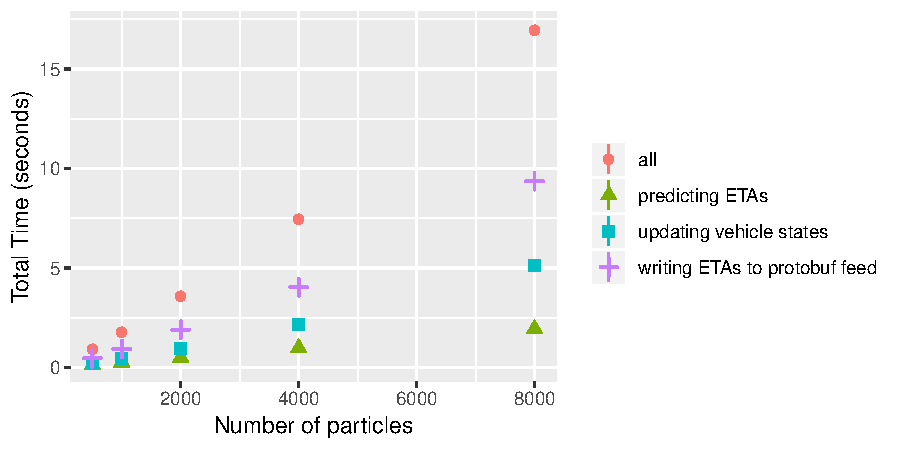
\includegraphics[width=0.8\textwidth]{figures/04_model_results_timing.pdf}
    \caption{
        The average real-time running time of each step within each iteration
        over a 15-minute off-peak window.
        The vehicle update and writing ETA steps involve sorting the particles,
        which is an operation of $\mathcal{O}(N\log N)$ complexity.
        Total time is for the entire iteration, which includes fetching the data from the API.
    }
    \label{fig:timings}
\end{figure}




\subsection{Model performance}
\label{sec:model_perf}


Evaluating the performance of the model involved
running the simulation using a range of values of GPS error, $\omega^2$,
and system noise, $\sigma^2$.
Figure \ref{fig:dist_to_route} shows the distribution of the distance
between each observation and the route using a nearest point algorithm,
which suggested using values $\omega \in \{1,2,3,5\}$ for GPS error in meters.
For the system noise, we used values of $\sigma^2\in \{1e^{-4},1e^{-3},1e^{-2},0.05\}$,
which correspond to an average vehicle speed variation of between 0.1 and 45~meters per second
over 30~seconds.
For each combination of these parameter values, including varying $N$,
the following values were calculated:
effective sample size, $N_\text{eff}$;
degeneration rate, the percentage of iterations in which the vehicle was lost
(no plausible particles remained);
and the (relative) variance of segment travel time estimates.


\begin{figure}[tb]
    \centering
    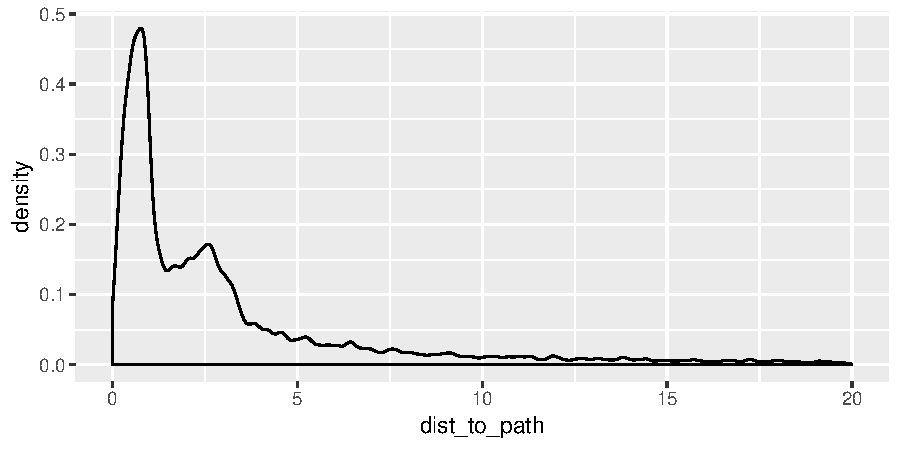
\includegraphics[width=0.7\textwidth]{figures/04_model_results_dist.pdf}
    \caption{
        The distribution of the minimum distance between observed vehicle location
        and the route path, truncated to 20~meters.
    }
    \label{fig:dist_to_route}
\end{figure}


\begin{figure}[tb]
    \centering
    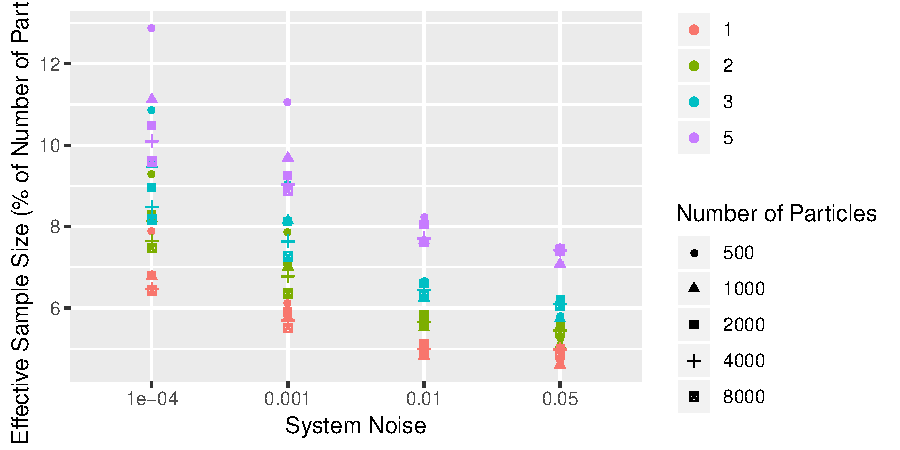
\includegraphics[width=\textwidth]{figures/04_model_results_neff.pdf}
    \caption{
        The effective sample size, $N_\text{eff}$,
        and degeneration rate for varying values of GPS error,
        system noise, and the number of particles $N$.
    }
    \label{fig:perf_stats}
\end{figure}


Figure~\ref{fig:perf_stats} shows that $N_\text{eff}$ increases
with GPS error and decreases with system noise
while remaining unaffected by changing $N$.
The degeneration rate decreases with GPS error and increases with $N$,
but is mostly unaffected by system noise.
Large GPS error affects the likelihood,
giving more weight to particles farther from the observation
than does a smaller GPS error.
Conversely, increasing system noise spreads out the particle cloud,
so fewer particles will be near the vehicle,
decreasing $N_\text{eff}$,
but more plausible trajectories are sampled,
so we see a slight decrease in degeneration rate.
Thus, these results are not surprising
and show that the model is working as expected.


The last measure of performance is the relative variance of segment travel times.
We used relative variance as each segment has a very different travel time distribution,
so to compare the variability between simulations we needed to
compute the average variance of estimated travel times over all simulations,
taking the average (over road segments) of the ratio between variance for
each simulation and variance over all simulations.
If $\tilde \bz_\ell^{\omega,\sigma}$ is a vector of all travel times
along segment $\ell$ during the simulation with GPS error $\omega$ and system noise $\sigma$,
then the relative variance $\bar v^{\omega,\sigma}$ is calculated by
\begin{equation*}
\begin{split}
v_\ell^{\omega,\sigma} &=
\frac{\mathrm{Var}(\tilde \bz_\ell^{\omega,\sigma})}{\mathrm{Var}(\tilde \bz_\ell)}, \\
\bar v^{\omega,\sigma} &=
    \frac{1}{L}\sum_{\ell=1}^L v_\ell^{\omega,\sigma}.
\end{split}
\end{equation*}
Figure~\ref{fig:travel_times} shows that simulations with larger GPS error
resulted in a higher relative variance,
while simulations with more particles had a smaller relative variance.
There was no clear pattern to the effect of system noise.


The results of the simulations
demonstrate a trade-off between particle filter performance
($N_\text{eff}$ and degeneration rate) and parameter estimation.
However, until the arrival time prediction model has been completed,
it is difficult to make decisions about the optimal values to use:
we are unable to say whether a higher variation of travel time estimates
is going to have a significant effect on the final ETAs,
particularly when compared to the uncertainty of forecasting road state.


\begin{figure}[tb]
    \centering
    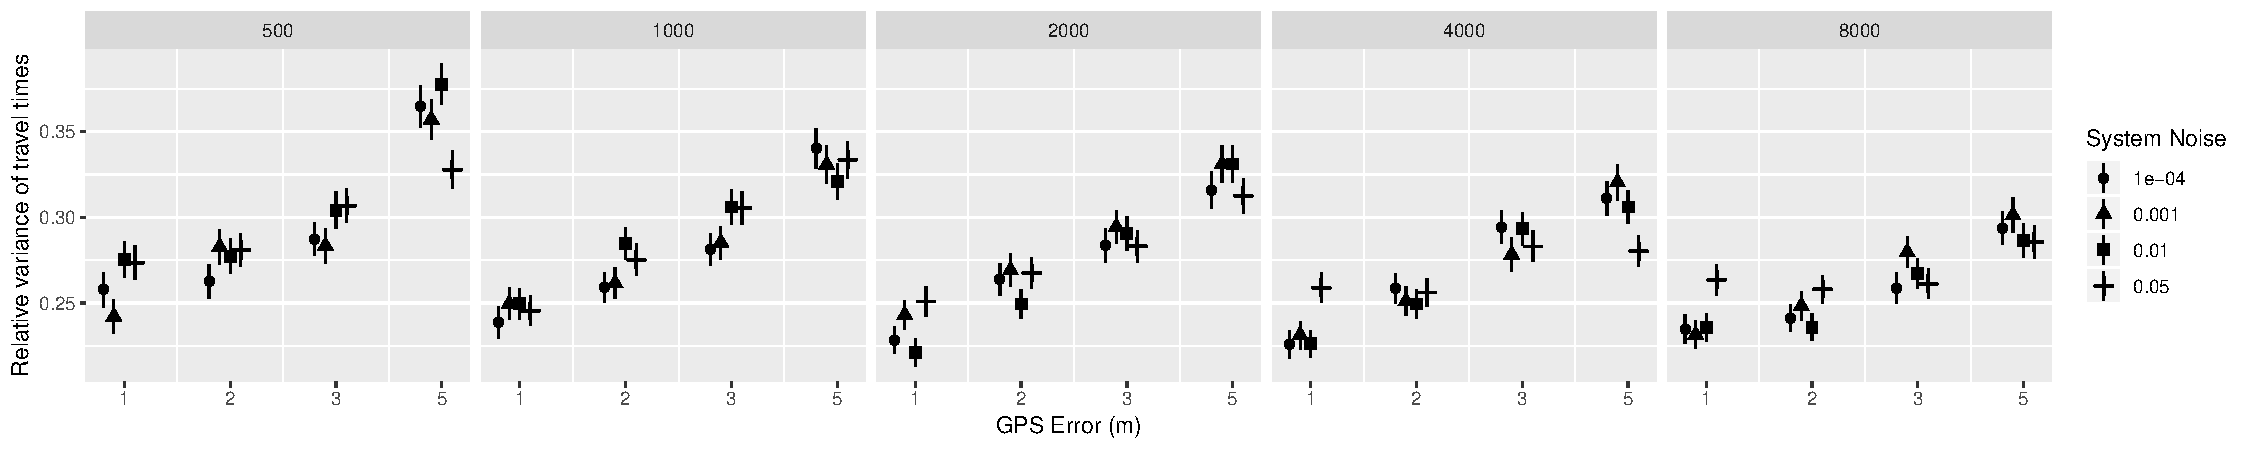
\includegraphics[width=\textwidth]{figures/04_model_results_times.pdf}
    \caption{
        The relative variability of travel time estimates for varying
        values of GPS error, system noise, and the number of particles, $N$,
        with error bars $\pm 2$ standard errors.
        % as GPS error increases,
        % with no clear relationship with system noise.
        % Increasing $N$ decreases variability.
    }
    \label{fig:travel_times}
\end{figure}


\section{Discussion and future work}
\label{sec:discussion}

In this paper, we described an approach to transit vehicle modelling
that enables the \rt estimation of road state from vehicle position data,
which will later be used to make arrival time predictions
that account for \rt traffic conditions.
The particle filter allows the modelling of complex bus behaviours,
providing estimates of vehicle travel times along roads
which are in turn used to estimate the road network state.


We have focussed on making a general framework
into which new models can be incorporated,
such as implementing intersection-specific behaviour
once intersection locations are available,
or exiting models changed.
For example, we plan to model stop dwell time using historical data,
which will allow us to replace the exponential distribution
with something more appropriate.


The network model presented here is simple,
but provides the foundation for future work to
develop a formal model combining \rt travel time information with historical data,
allowing short- and medium-term forecasts of road state,
for example incorporating peak time congestion.
As for the arrival times,
we plan to estimate these from a combination of historical
and \rt data.
The model presented in this paper provides the starting point
for a transit modelling and predictive framework
that can be adapted to specific transit providers,
combined with historical data,
and run in \rt to provide commuters with
improved ETAs with which they can more reliably
plan their commutes.


The results of our simulations show that the framework is a
feasible \rt alternative.
While the timings presented were for off-peak times,
further investigation into the choice of $N$ and $N_\text{eff}$,
as well as work removing redundancy from the transition algorithm,
should allow us to model all vehicles during peak periods---%
when there are 2--3~times as many vehicles---%
within our 30-second time frame target.


\bibliographystyle{anzsj}
\bibliography{reflist.bib}

\end{document}
